\setlength{\parskip}{1em}

\chapter{Zadání}

Cílem semestrální práce je naučit se implementovat komplexní systém s využitím hotových knihoven pro preprocessing. Vedlejším produktem bude hlubší porozumnění indexerům, vyhledávacím systémům a přednáškám.
Systém po předchozím předzpracování zaindexuje zadané dokumenty a poté umožní vyhledávání nad vytvořeným indexem. Vyhledávání je možné zadáním dotazu s logickými operátory AND, OR, NOT. Výsledek dotazu by měl vrátit top x (např. 10) relevantních dokumentů seřazených dle relevance.\\
Projekt by měl být implementován v jazyce Java s využitím poskytnutých podpůrných interfaců a abstraktních tříd. Výstupem bude jeden jar soubor obsahující javaDoc, přeložené i zdrojové soubory projektu a dokumentace popisující jednotlivé funkčnosti semestrální práce s důrazem kladeným na nadstandardní funkčnosti a vlastní řešení.
Semestrální práce se bude testovat indexací dokumentů a vyhledáváním relevantních dokumentů nad vytvořeným indexem (tyto data nesmíte dále šířit a používat pro jiné účely). Pro porovnání jednotlivých semestrálních prací mezi sebou bude nakonec zveřejněna tabulka s naměřenými hodnotami. Proto je třeba aby váš projekt obsahoval třídy z projektu Interface (při doplnění Třídy Index lze spuštěním TestTrecEval získat výsledný soubor (relevantní dokumenty) a pokud lze spustit evaluační skript (trec\_eval.8.1/trec\_eval) tak výsledek evaluace (popis viz README). Hlavní evaluační metrika je Mean Average Precision (MAP). Pomocí této hodnoty budeme řadit vaše výsledky. Pokud nechcete zveřejnit své výsledky, dejte nám to vědět emailem.


%%%%%%%%%%%%%%%%%%%%%%%%%%%%%%%%%%%%%%%%%%%%%%%%%%%%%%%%%%%%%%%%%%%%%%%%%%%%%%%%%%%%%%%%%%%%%%%%%%%%

\chapter{Indexace}
Při indexaci projde každý dokument nejprve preprocessingem. Poté se vytvoří invertovaný index a spočte tf-idf váha. Dokumenty se mouhou doindexovat i zpětně, připadně aktualizovat nebo odebrat.

\section{Preprocessing}
Nejprve se text převede na lower case.  Poté se text tokenizuje, jako první datumy, webové adresy a odstraní se html tagy. Pak se provede stemming a odstraní se akcenty. Na závěr se odstraní stop slova.

\section{Inverted index}
Inverted index představuje Hash mapa. Klíč je term, hodnota je seznam dokumentů, ve kterých se term vyskytuje a s jakou frekvencí.

\section{Tf-idf}
Tf-idf je metodika hodnocení relevance při vyhledávání textu. Tf-idf hodnota pro každý term v dokumentu je spočtena jako tf*idf, kdy tf je četnost slova v dokumentu a idf je převrácená četnost slova ve všech dokumentech.

\begin{figure}[h]
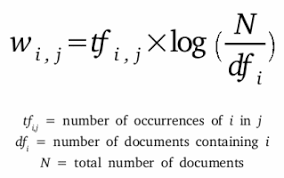
\includegraphics[width=5cm]{tfidf}
\centering
\end{figure}


%%%%%%%%%%%%%%%%%%%%%%%%%%%%%%%%%%%%%%%%%%%%%%%%%%%%%%%%%%%%%%%%%%%%%%%%%%%%%%%%%%%%%%%%%%%%%%%%%%%%

\chapter{Vyhledávání}
Při vyhledávání se query nejprve tokenizuje (projde preprocessingem stejně jako při indexci). Následně se vytvoří seznam termů pro logické operace AND/OR/NOT (operandy se z query odstraní). Vypočte se tf-idf váhový vektor a jeho normalizovaný tvar.\\

Pro každý dokument, který obsahuje term z query se vytvoří tf-idf váhový vektor. Pokud dokument některý term neobsahuje, je na dané pozici vektoru 0. Poté se provedou logické operace AND/OR/NOT. Následně se všechny váhové vektory normalizují.\\

Nakonec se pro každý dokument vypočte skóre, výsledky se seřadí od největšího skóre a ohodnotí.

\section{Logické operace AND/OR/NOT}
Každý dokument se vyhodnotí podle seznamu logických operátorů AND/OR/NOT. Nevyhovující dokument se z výsledků odstraní.\\
\\
AND - v dokumentu musí být obsaženy oba termy (tj hodnota vektoru na pozici daných termů je nenulová)\\
OR - v dokumentu musí být obsažen alespoň jeden z termů\\
NOT - daný term nesmí být v dokumentu obsažen\\
\\
Pokud by po provedení logických operací nezbyl žádný dokument, logické operace se neprovedou.\\ \\ \\

\section{Výpočet skóre}
Skóre se vypočte pomocí cosine similarity. Provede se skalární součin váhového vektoru query a dokumentu, který se vydělí součinem jejich normalizovaných tvarů.

\begin{figure}[h]
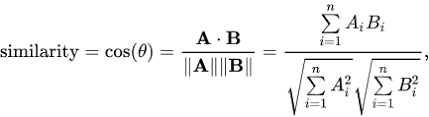
\includegraphics[width=8cm]{cosine}
\centering
\end{figure}

%%%%%%%%%%%%%%%%%%%%%%%%%%%%%%%%%%%%%%%%%%%%%%%%%%%%%%%%%%%%%%%%%%%%%%%%%%%%%%%%%%%%%%%%%%%%%%%%%%%%

\chapter{Spuštění}

Aplikace se spouští příkazem \textbf{java jar Indexer.jar [path]}\\
Evaluace se spouští příkazem \textbf{java jar IndexerEval.jar}
\\
\\
Ovládání aplikace  \textbf{Indexr.jar} po načtení dat:\\
\begin{tabular}{ l l l }
q & query\\
a & path & add document\\
u &  path & update document\\
r & docId & remove document\\
h && help\\
e && exit
\end{tabular}
\\
\\
Pro spuštění je potřeba mít nainstalovanou javu 1.8.\\
V adresáři, kde se nachází jar soubor, musí být soubor \emph{stopwords.txt}, který obsahuje stop slova, adresář \emph{TREC} s daty \emph{czechData.bin} a \emph{topicData.bin}. Do tohoto adresáře se ukládají výsledky. Pro spuštění evaluace musí být adresář \emph{trec\_eval.8.1} s evaluační aplikací.


%%%%%%%%%%%%%%%%%%%%%%%%%%%%%%%%%%%%%%%%%%%%%%%%%%%%%%%%%%%%%%%%%%%%%%%%%%%%%%%%%%%%%%%%%%%%%%%%%%%%

\chapter{Výsledky evaluace}

\begin{center}
\begin{tabular}{ l l l l l}

num\_q      &&     all &&    50\\
num\_ret     &&    all  &&   3719126\\
num\_rel     &&    all   &&  762\\
num\_rel\_ret &&    all&&     760\\
map        &&     all     &&0.1804\\
gm\_ap      &&     all   &&  0.0527\\
R-prec        &&  all    && 0.1999\\
bpref         &&  all     &&0.1842\\
recip\_rank   &&   all  &&   0.4056\\
ircl\_prn.0.00  && all &&    0.4480\\
ircl\_prn.0.10  && all &&    0.3453\\
ircl\_prn.0.20  && all &&    0.2870\\
ircl\_prn.0.30  && all &&    0.2534\\
ircl\_prn.0.40  && all &&    0.2203\\
ircl\_prn.0.50  && all &&    0.1891\\
ircl\_prn.0.60  && all &&    0.1600\\
ircl\_prn.0.70  && all &&    0.1291\\
ircl\_prn.0.80  && all &&    0.1025\\
ircl\_prn.0.90  && all &&    0.0560\\
ircl\_prn.1.00  && all &&    0.0478\\
P5           &&   all   &&  0.2480\\
P10          &&   all  &&   0.1920\\
P15          &&   all  &&   0.1707\\
P20          &&   all  &&   0.1540\\
P30          &&   all  &&   0.1347\\
P100        &&    all &&    0.0652\\
P200        &&    all &&    0.0394\\
P500        &&    all &&    0.0202\\
P1000      &&     all&&     0.0112

\end{tabular}
\end{center}



%%%%%%%%%%%%%%%%%%%%%%%%%%%%%%%%%%%%%%%%%%%%%%%%%%%%%%%%%%%%%%%%%%%%%%%%%%%%%%%%%%%%%%%%%%%%%%%%%%%%

\chapter{Závěr}
V rámci semestrální práce jsem implementoval poždovanou základní funkcionalitu a některou nadstandardní.\\
Evaluaci jsem spustil na ZČU serveru ares.fav.zcu.cz. Mean Average Precision (MAP) při evaluaci vyšlo 0.1804.
\\
\\
\setlength{\parskip}{0em}
\textbf{Implementovaná nadstandartní funkčnost:}
\begin{itemize}
\item ošetření html tagů
\item tokenizace datumů
\item doindexování dokumentů
\item dokumentace v LaTeXu
\end{itemize}
